\documentclass[12pt]{article}
\usepackage[utf8]{inputenc}
\usepackage[left=2cm,right=2cm,top=2cm,bottom=2cm]{geometry}
\usepackage[spanish]{babel}
\usepackage{graphicx, amsmath}
\usepackage[small]{caption}
\usepackage{subcaption, enumerate}
\usepackage{url}
\setlength{\parskip}{\baselineskip}
%\setlength{\parskip}{0.3cm}
\graphicspath{ {images/} }
\allowdisplaybreaks

\spanishdecimal{.}

\usepackage{hyperref}
\hypersetup{
	colorlinks=true,
	linkcolor=blue,     
	urlcolor=blue,
	citecolor=blue,
}

\newtheorem{theorem}{Teorema}


\begin{document}

	\thispagestyle{empty}

	\begin{center}
		{\Large \bf Teorema del límite central}\\
		Gabriela S\'anchez Y.\\
		5064
	\end{center}
  
  	\section{Teorema del límite central}
  	
	El teorema del límite central es otro de los teoremas fundamentales de la probabilidad. El enunciado formal de acuerdo a Grinstead y Snell \cite{prob2003} es el siguiente.
	
	\begin{theorem}[Teorema del límite central ]
		Sea $X_1, X_2, \ldots, X_n$ una secuencia de variables aleatorias independientes e idénticamente distribuidas y sea $S_n = X_1 + X_2 + \ldots + X_n$. Para cada $n$ la media y varianza de $X_n$ se denotan por $\mu_n$ y $\sigma_n^2$, respectivamente. Defina la media y varianza de $S_n$ como $m_n$ y $s_n^2$, respectivamente y asuma que $s_n \rightarrow \infty$. Si existe una constante $A$ tal que $|X_n| \leq A$ para todo $n$, entonces para $a<b$,
		\begin{equation*}
		\lim_{n \rightarrow \infty} P \left( a < \frac{S_n - m_n}{s_n} < b  \right) = \frac{1}{\sqrt{2\pi}} \int_{a}^{b} e^{x^2/2} \, dx.
		\end{equation*}
	\end{theorem}

	En esencia lo que el teorema dice es que el promedio de las medias de muestras será la media de la población. Es decir, si se suman las medias de todas las muestras y se determina el promedio, ese promedio será la media de la población real.

	
	\section{Aplicaciones}
	
	%Algunas de las aplicaciones prácticas del teorema central del límite en aprendizaje máquina 
	%Si se tiene una muestra que sea representativa de toda la población, el teorema del límite central ayuda a hacer inferencias acerca de los parámetros de la muesta y de la población 

	\subsection{Experimentación con datos de la tesis}
	
	Se tienen soluciones de un modelo con dos métodos distintos. Uno de ellos, un optimizador y el otro una metaheurística. Para cada resultado se hace una comparación para saber qué tan alejados están uno del otro, tomando como base el valor obtenido por el optimizador. En otras palabras, se calcula un gap de la siguiente manera
	\begin{equation*}
	gap = \frac{z_{opt} - z_{met}}{z_{opt}} \times 100 \%,
	\end{equation*}
	en total se tienen 3510 resultados y se desea saber si habría un comportamiento tal y como lo dice el teorema.
	
	Se toman cien muestras de tamaño $n$ variable, con $n=30$, 50 y 80. La distribución que tienen las medias de las muestras se puede observar en los histogramas de la figura \ref{gaps}.
	
	\begin{figure}
		\begin{subfigure}{\textwidth}
			\centering
			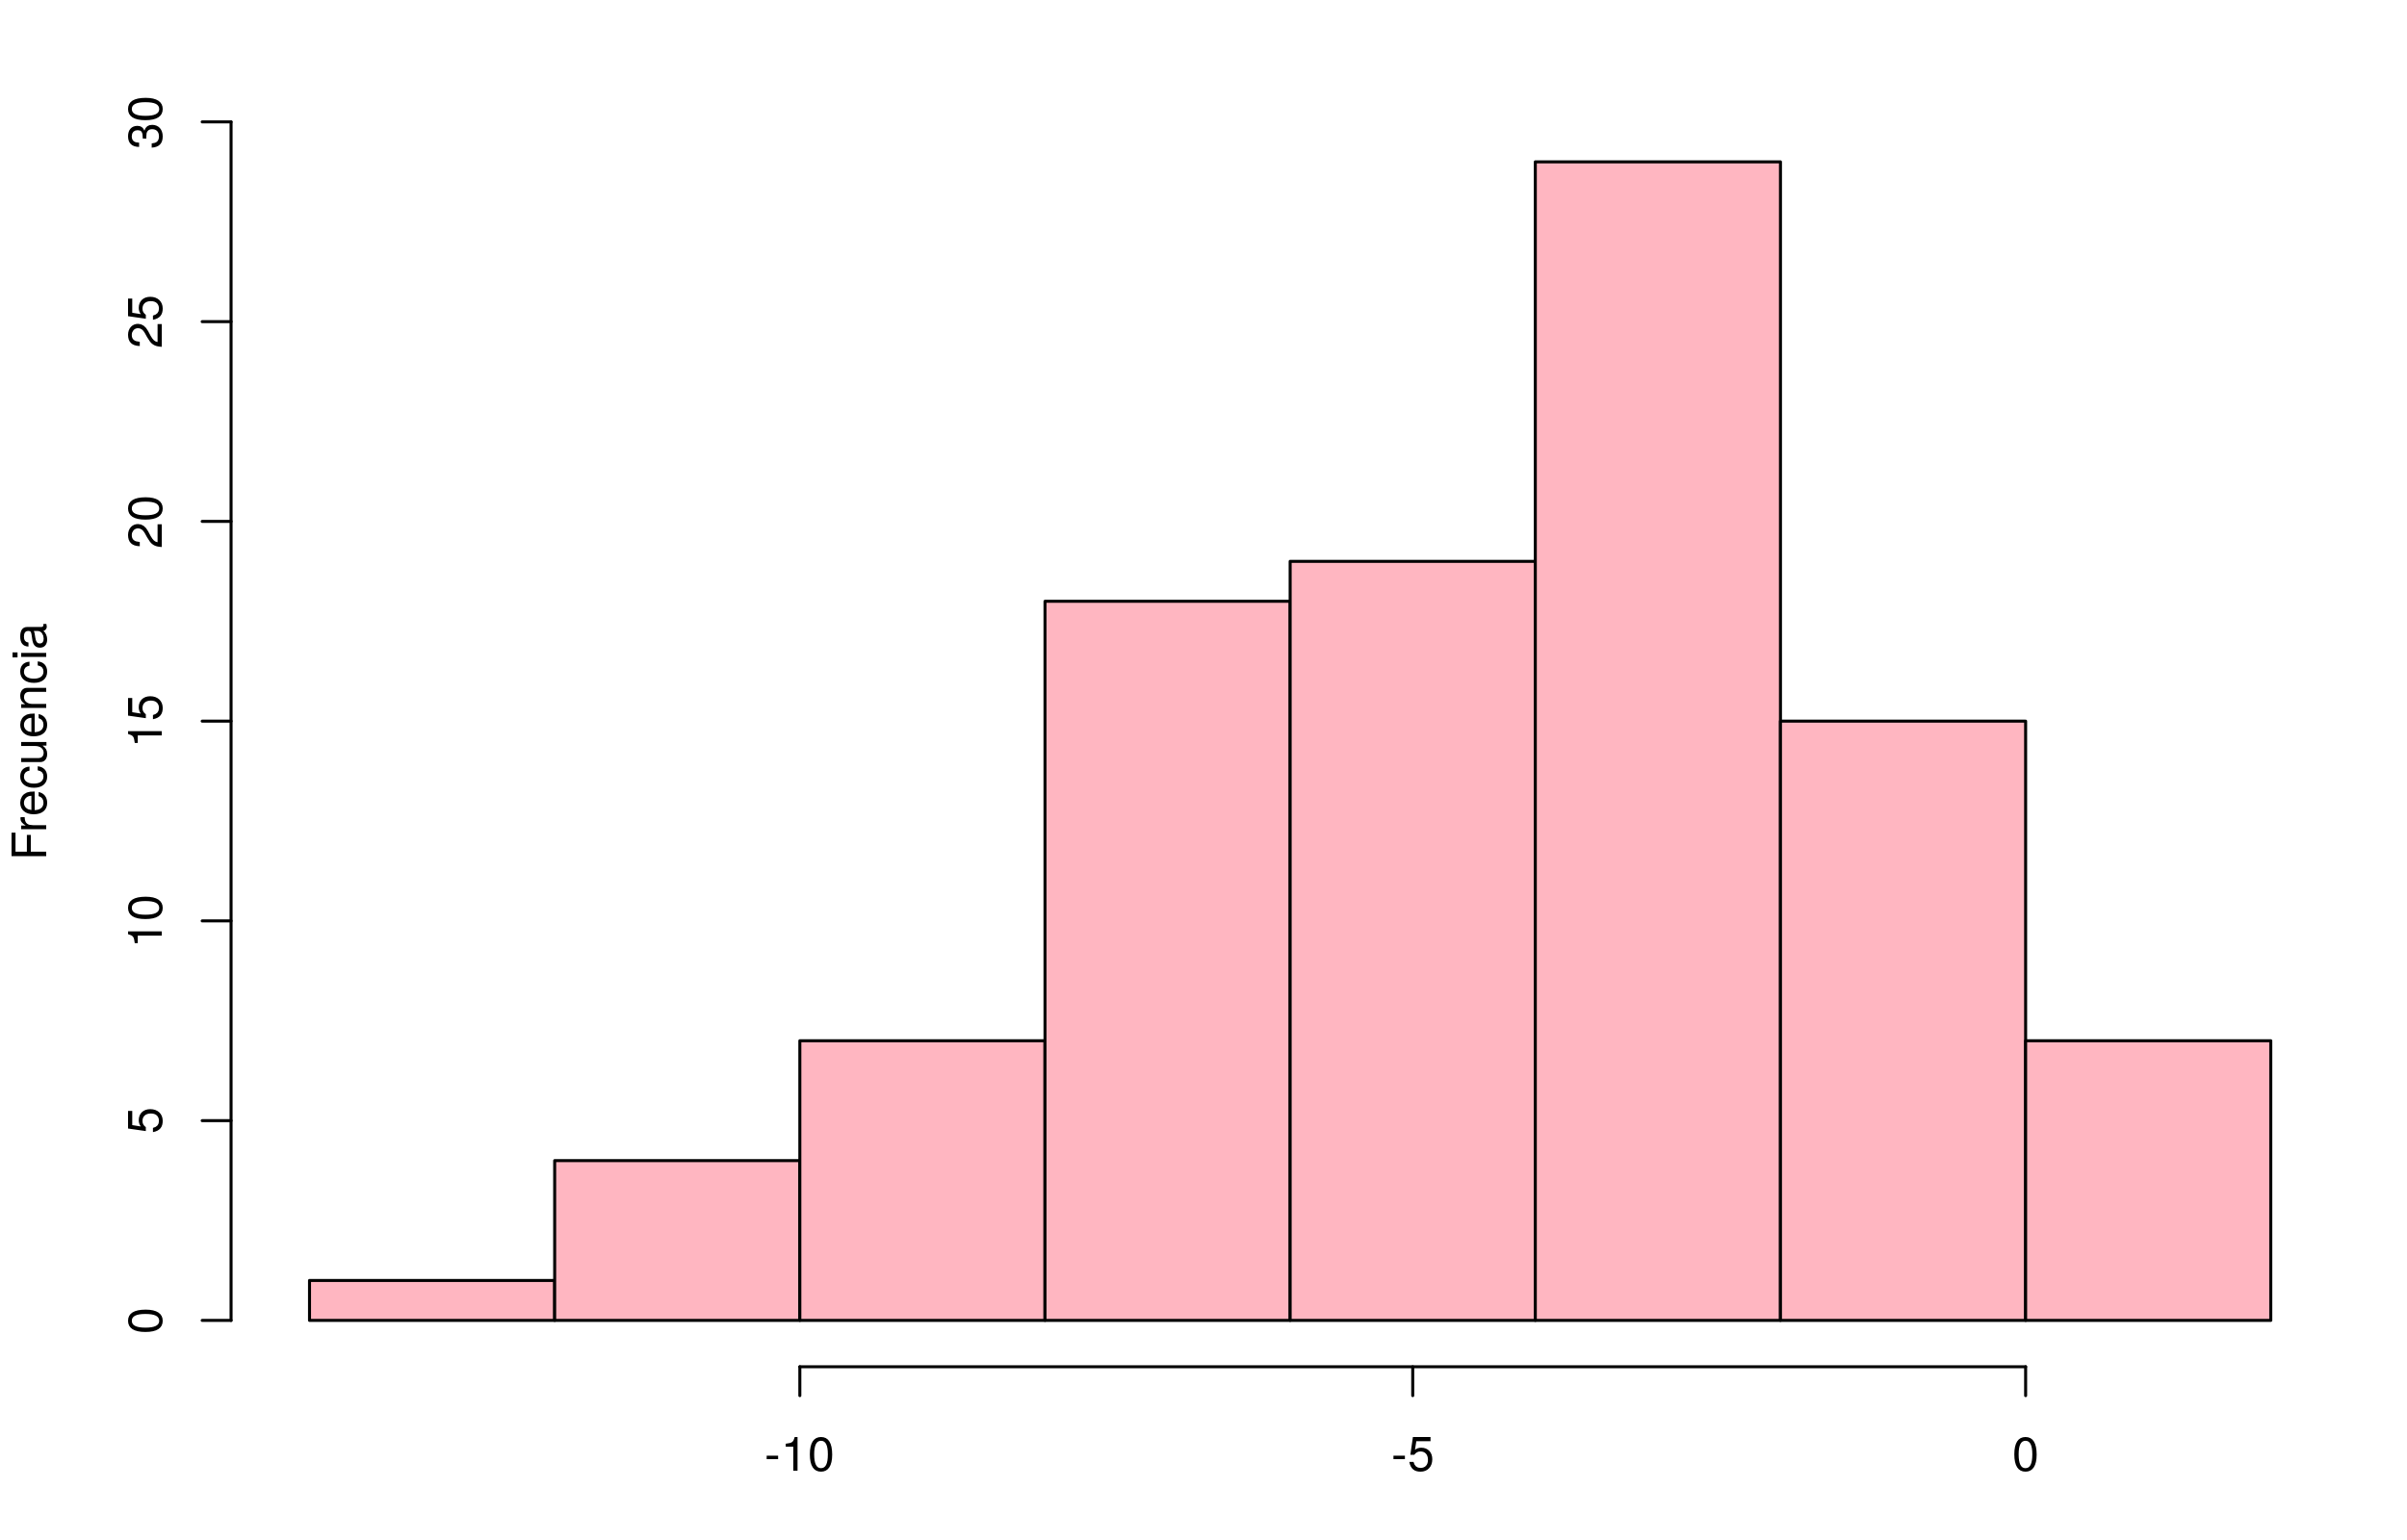
\includegraphics[scale=0.5]{meangap_10.png}
			\caption{$n=10$}
		\end{subfigure}
	
		\begin{subfigure}{\textwidth}
			\centering
			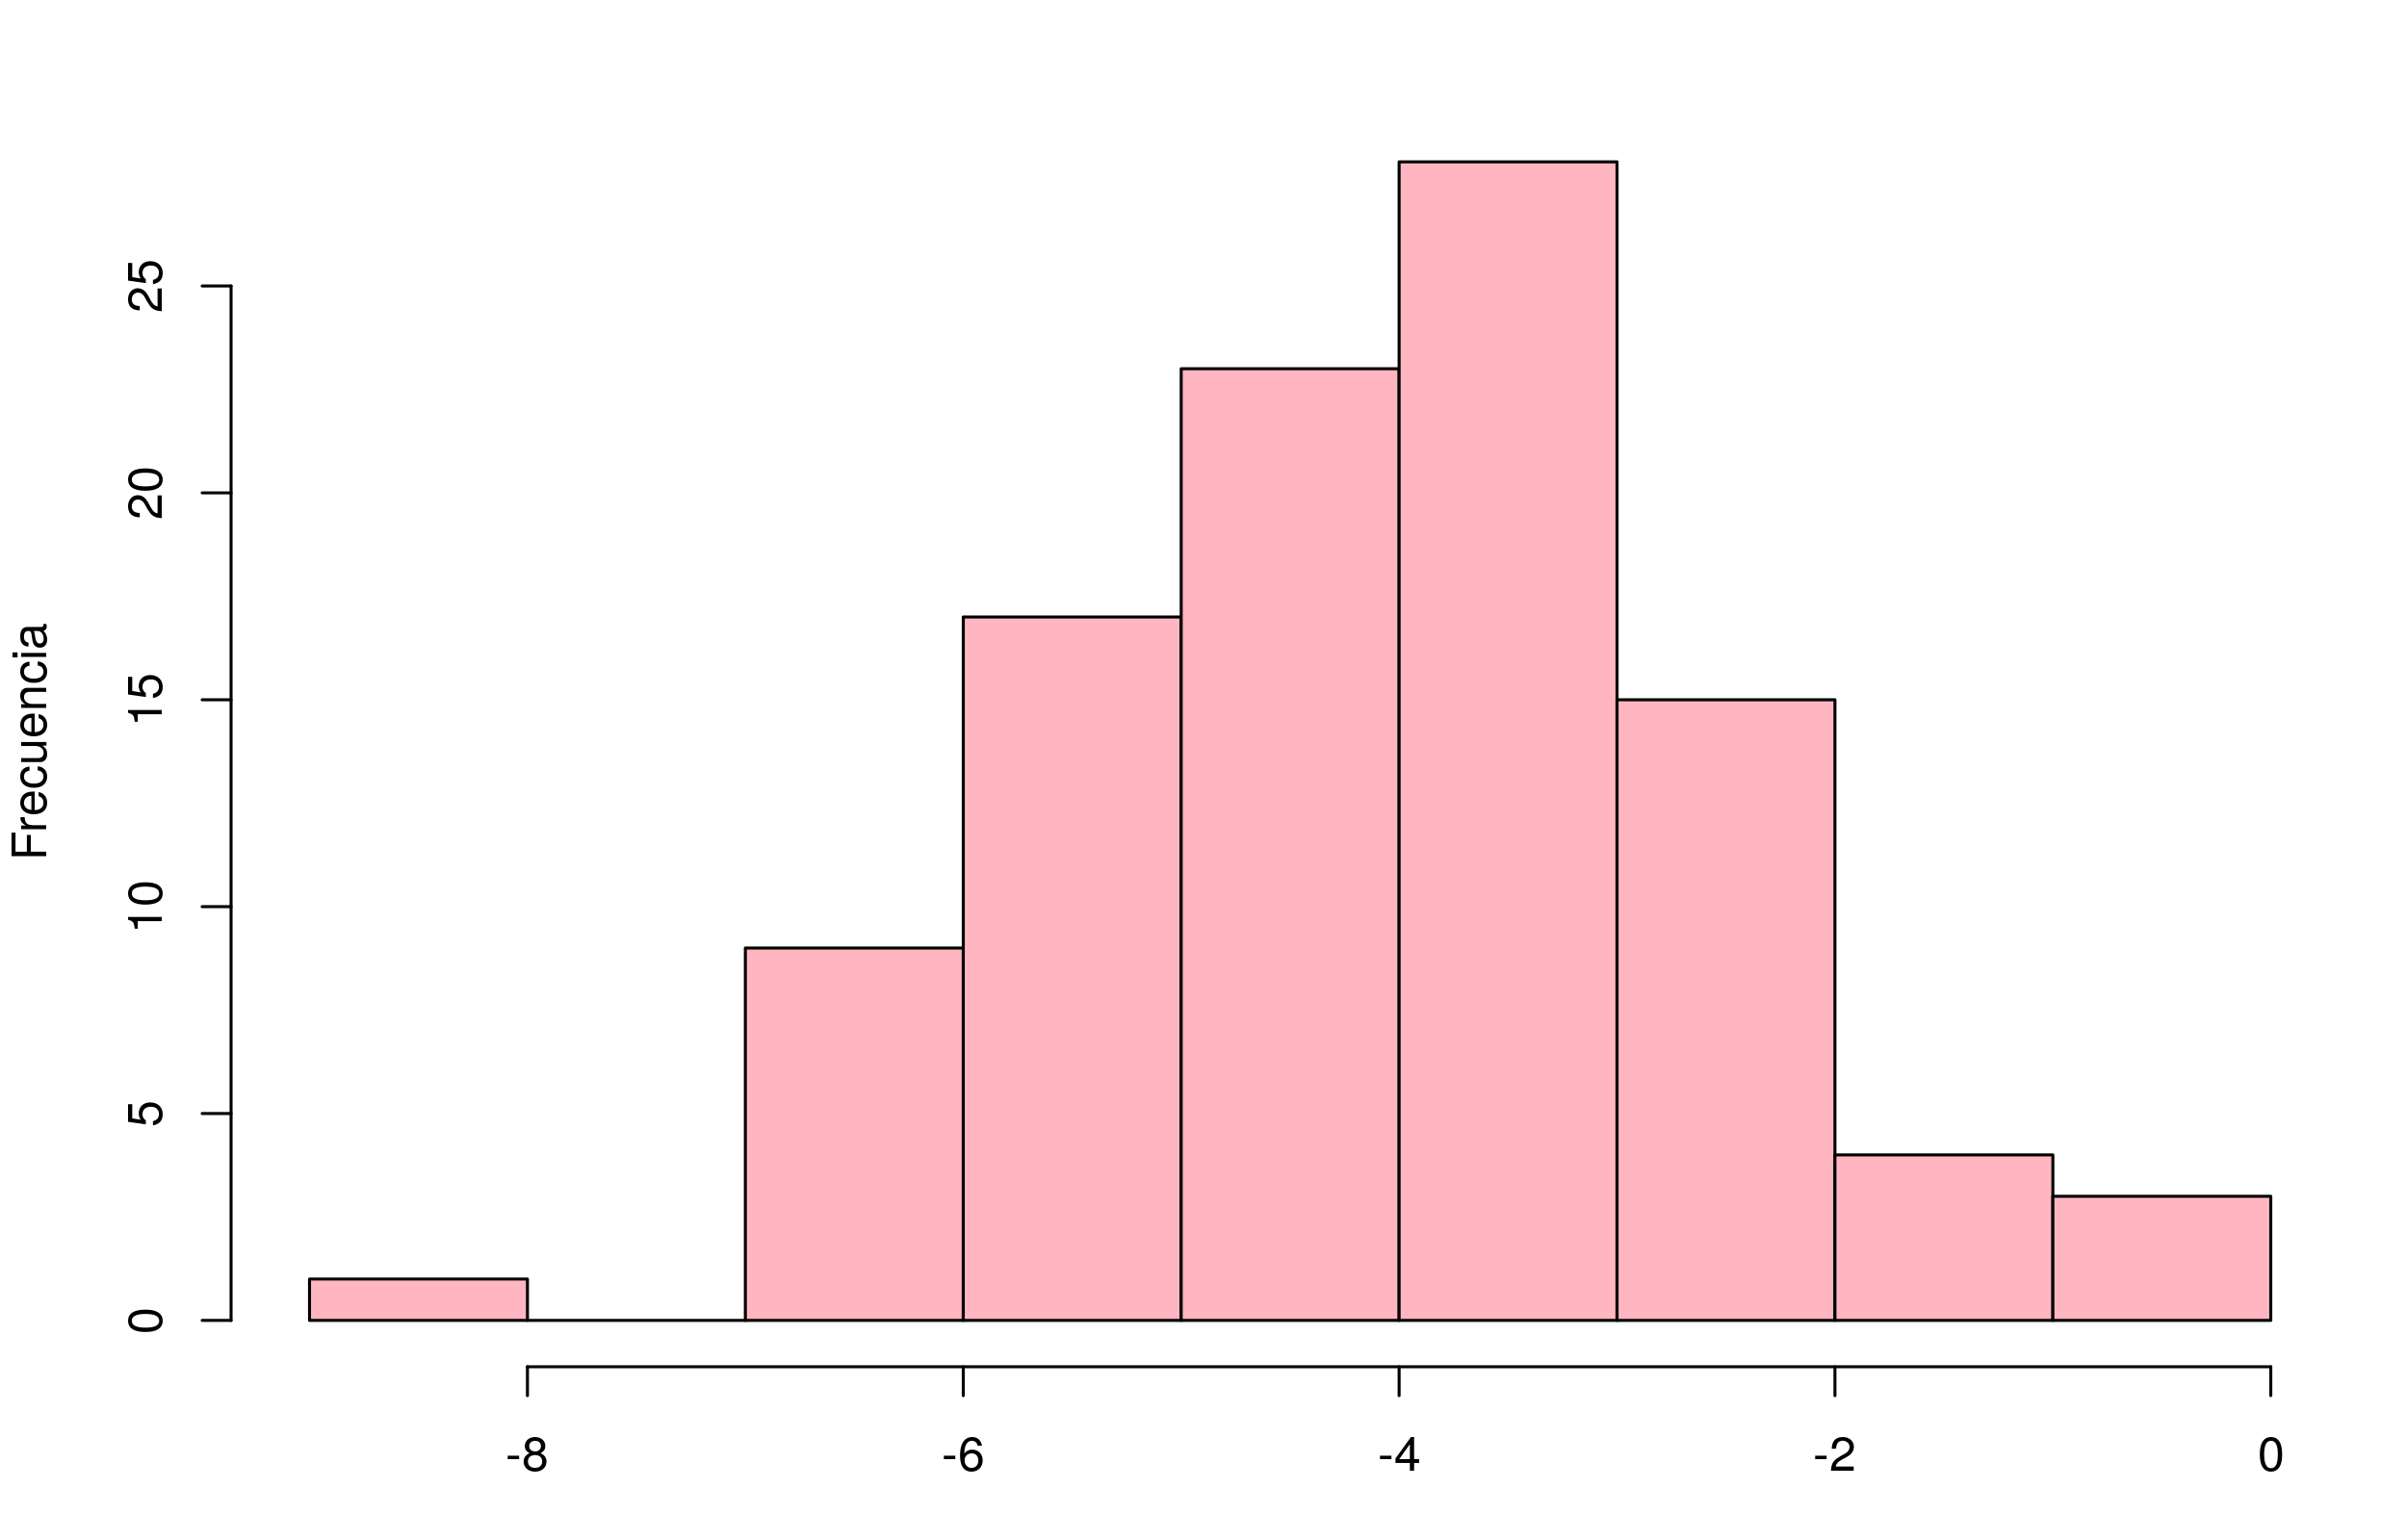
\includegraphics[scale=0.5]{meangap_50.png}
			\caption{$n=50$}
		\end{subfigure}
	
		\begin{subfigure}{\textwidth}
			\centering
			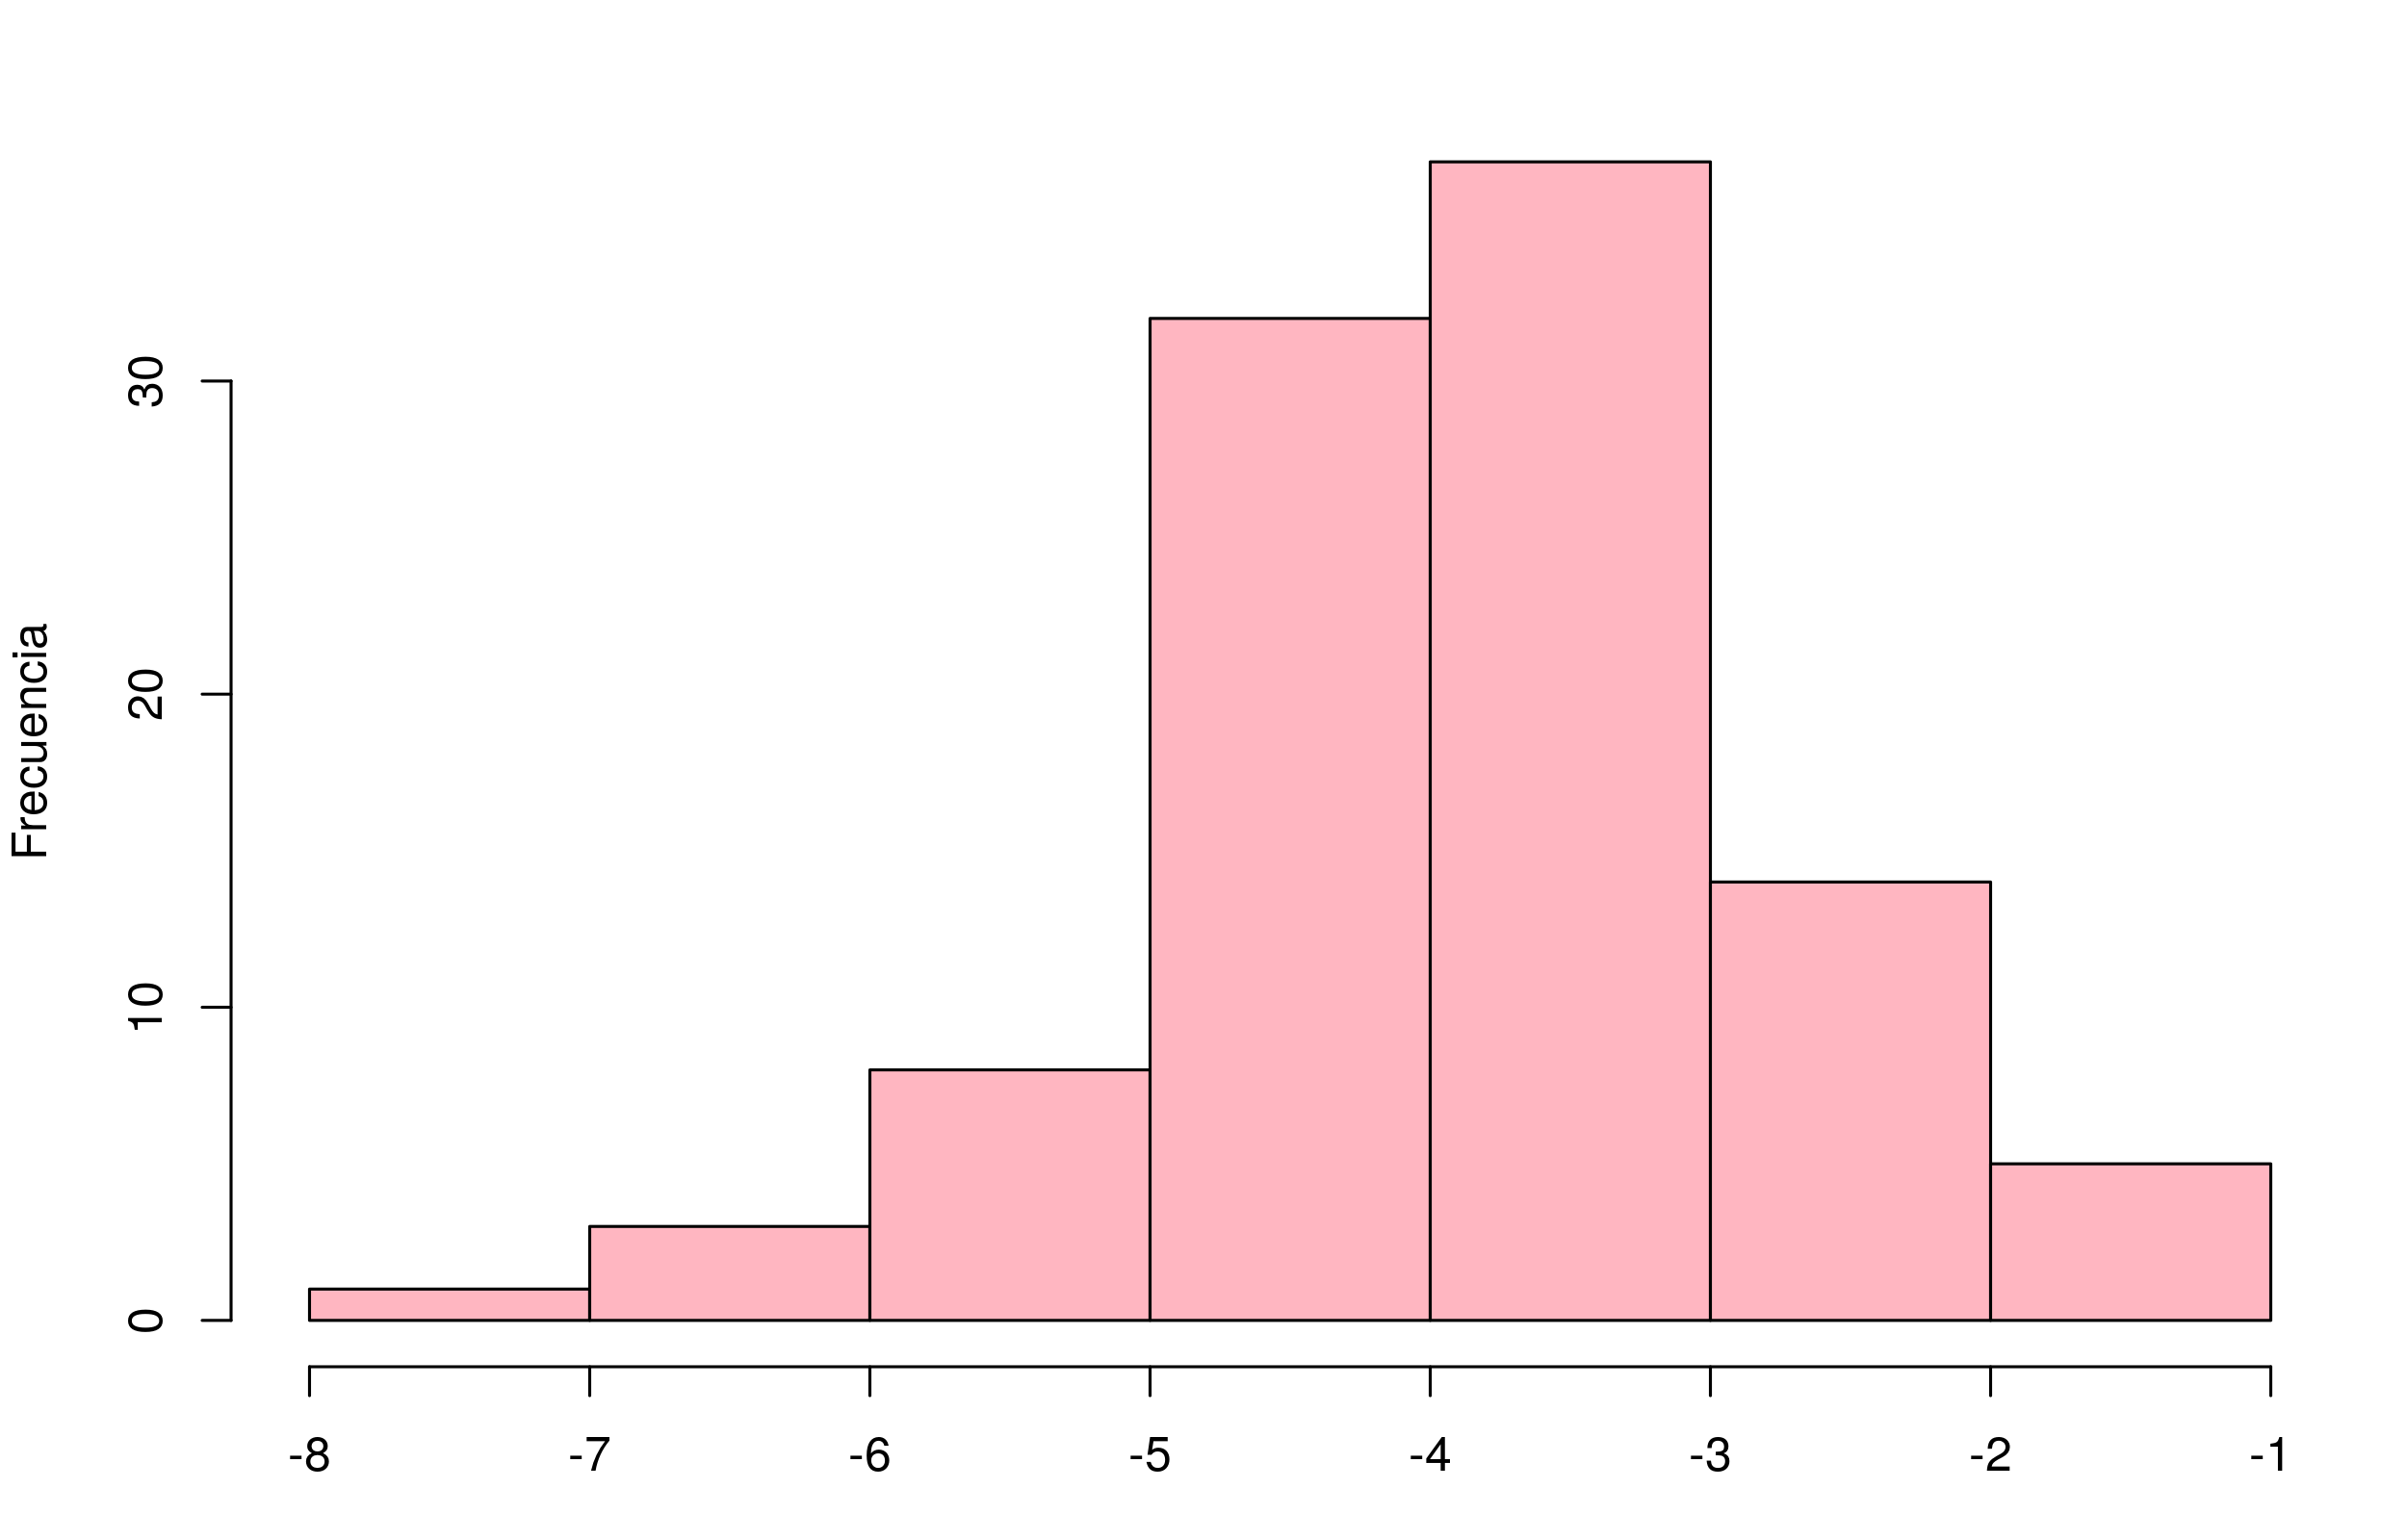
\includegraphics[scale=0.5]{meangap_80.png}
			\caption{$n=80$}
		\end{subfigure}
	\caption{Distribución de las medias de cien muestras de tamaño variable.}
	\label{gaps}
	\end{figure}
	
\bibliographystyle{plain}
\bibliography{biblio}

\end{document}
